\documentclass[12pt,a4paper,utf8]{ctexart}
\usepackage{ctex,amsmath,amssymb,subfig,cite,graphicx,diagbox,fontspec,fancyhdr,geometry}
\usepackage[ntheorem]{empheq}
\usepackage{enumitem,fullpage,cleveref,cellspace,listings,color,framed}
\definecolor{gray}{rgb}{0.5,0.5,0.5}
\definecolor{dkgreen}{rgb}{.068,.578,.068}
\definecolor{dkpurple}{rgb}{.320,.064,.680}

%set Fortran styles
\lstset{
    frameround=tftf,
    language=Fortran,
    keywords={SELECT,PROGRAM,PRINT,STOP,END,WRITE,INTEGER,REAL,COMPLEX,CHARACTER,LOGICAL,READ,FORMAT,IMPLICIT,PARAMETER,DATA,EQUIVALENCE,TYPE,PAUSE,CONTINUE,CYCLE,EXIT,IF,SELECT,DO,ALLOCATE,DEALLOCATE,WHERE,FORALL,SUBROUTIHNE,CALL,RETURN,FUNCTION,COMMON,BLOCK DATA,SAVE,INTERFACE,CONTAIN,MODULE,USE,PUBLIC,PRIVATE,ENTRY,OPEN,INQUIRE,CLOSE,NAMELIST,POINTER,NULLFY,REWIND,BACKSPACE,ENDFILE
    },
    basicstyle=\small\ttfamily,
    numbers=left,
    numberstyle=\small,
    keywordstyle=\color{blue}\bfseries,
    commentstyle=\color{dkgreen},
    stringstyle=\color{dkpurple},
    backgroundcolor=\color{white},
    tabsize=2,
    showspaces=false,
    showstringspaces=false,
    breaklines=true,
    frame=trBL,
}
\CTEXsetup[format+={\raggedright}]{section}
\setlength{\parindent}{2em}
\geometry{
    textwidth=138mm,
    textheight=215mm,
    left=27mm,
    right=27mm,
    top=25.4mm,
    bottom=25.4mm,
    headheight=2.17cm,
    headsep=4mm,
    footskip=12mm,
    heightrounded,
}
\pagestyle{fancy}
\lhead{\textsl{2021秋-计算物理A}}
\chead{}
\rhead{\textsl{PB19020634-于浩然}}
\lfoot{}
\cfoot{\thepage}
\rfoot{}

\begin{document}
\begin{center}
    {\LARGE\textbf{计算物理作业三}}\\
    \textrm{于浩然}~~~~~~\textrm{PB19020634}~~~~~~\textrm{2021.10.16}
\end{center}
\section{作业题目}

在球坐标系$(\rho, \theta,
\varphi)$下,产生上半球面上均匀分布的随机坐标点,给出其直接抽样方法.

\section{算法简介}

\subsection{直接抽样方法}
对于连续型变量的直接抽样方法,我们考虑如下量,将其称为累积函数:
\begin{equation}
    \xi (x) = \int_a ^x p(x') \textrm{d}x'  
\end{equation}

其中 $p(x)$是已经归一化的几率密度分布函数,定义为:
\begin{equation}
    \int _a ^b p(x) = 1, \quad p(x) \geq 0 
\end{equation}
\begin{equation}
    \textrm{d} P(x \rightarrow x + \textrm{d} x) = p(x) \textrm{d} x
\end{equation}

上式中 $P$为无量纲几率,几率密度函数 $p(x)$的量纲为自变量量纲的倒数.

我们只需由累积函数 $\xi (x)$的表达式反解出
$x(\xi)$的函数表达式,即求反函数,这样就得到了几率密度分布 $p(x)$的直接抽样方法.

\subsection{本题具体解法}

我们首先需要定义球坐标系 $(\rho, \theta,
\varphi)$中单位球面上的“均匀分布”,可理解为在相同面积元 $
\textrm{d}S = \sin \theta \textrm{d} \theta \textrm{d} \varphi$上取点的概率 $ \textrm{d}P$均相同,可表达如下式:
\begin{equation}
    \textrm{d} P = p(\theta,\varphi) \textrm{d} \theta \textrm{d}
    \varphi = p(\theta,\varphi) \textrm{d}S / \sin \theta
\end{equation}
\begin{equation}
    \frac{ \textrm{d}P}{ \textrm{d}S} = \frac{p( \theta, \varphi)}{\sin \theta}
    = const.
\end{equation}

为满足上述关系,我们不妨设$p(\theta, \varphi) = k \sin \theta $ ($k$为常数)

上半球面有$0 \leq \theta \leq \pi /2$,$0 \leq \varphi
\leq 2\pi$由归一化关系:
\begin{equation}
    \iint p(\theta, \varphi) \textrm{d} \theta \textrm{d} \varphi = \int_0 ^{2
    \pi} \int _0 ^{\pi / 2} k \sin \theta \textrm{d} \theta \textrm{d} \varphi =
   2\pi k =1
\end{equation}

因此我们得到$k=1/2\pi$,
\begin{equation}
p(\theta, \varphi)=\sin \theta / 2\pi
\end{equation}

由于均匀分布的独立性,$\theta$和$\varphi$应相互独立,我们不妨设$p(\theta,
\varphi)=p(\theta)p(\varphi)$. 除了$(\theta,
\varphi)$的联合密度归一化外,$p(\theta)$和$p(\varphi)$必须分别满足几率密度函数归一化:

\begin{equation}
    \int _0 ^{\pi /2} p(\theta) \textrm{d} \theta = 1 , \qquad \int _0 ^{2\pi} p(\varphi) \textrm{d} \varphi = 1 
\end{equation}

容易得到:
\begin{equation}
    p(\theta)=\sin \theta , \qquad p(\varphi)=1/2\pi
\end{equation}

分别求累积函数$\xi(\theta)$和$\eta(\varphi)$:
\begin{eqnarray}
    \xi(\theta) &=& \int _0 ^{\theta} \sin \tau \textrm{d} \tau = 1 - \cos
    \theta \\
    \eta(\varphi) &=& \int _0 ^{\varphi} 1/2\pi \textrm{d} \tau =
    \frac{\varphi}{2\pi}
\end{eqnarray}

求解反函数:
\begin{eqnarray}
    \theta(\xi) &=& \arccos (1 - \xi) \rightarrow \arccos \xi \\
    \varphi(\eta) &=& 2\pi \eta
\end{eqnarray}

其中由于$1- \xi$也服从均匀分布,故直接将其替换为$\xi$.这样,我们便可以通过$[0,1]$上均匀分布的两个随机数序列$\xi$和$\eta$利用上式产生上半球面上均匀分布的随机数点.

\section{编程实现}

本题中我们需要使用随机数产生器,为方便起见考虑使用以前编程实现过的16807生成器,使用两个不同的种子生成两组一定数目的随机数,再使用(12)(13)式生成单位上球面$\rho=1,z>0$上的均匀随机数点.

使用Fortran90进行编程,程序各部分及其功能介绍如下:
\begin{itemize} 
    \item \texttt{PROGRAM MAIN}\\
        在主程序中,使用
        \texttt{DO}循环结构考察随机数数目分别为$10^3,10^4,10^5$时的情况,让整型变量
        \texttt{intI}分别为3、4和5. 这里使用了一个小技巧,用
        \texttt{WRITE}语句把整型量
        \texttt{intI}转变为字符型量
        \texttt{charI},以便写入文件名便于后续区分和使用. 对于每个
        \texttt{intI}值,(手滚键盘)输入两个随机数种子来生成两组随机数序列,再调用
        \texttt{Sphererd}子程序进行直接抽样,得到不同数目的$(\theta,
        \varphi)$均匀分布序列,最后储存在文件中.

\begin{framed}
\begin{lstlisting}[language=Fortran]
PROGRAM MAIN
    INTEGER(KIND=4) :: intI
    CHARACTER(LEN=1) :: charI
    DO intI = 3, 5
        WRITE (charI,"(I1)") intI !此语句将10以内的整型数据intI变为字符类型charI
        CALL Schrage(intI, 1651661, 'x'//charI//'.dat')
        CALL Schrage(intI, 7459556, 'y'//charI//'.dat')
        CALL Sphererd(intI) !使用前面生成的随机数进行抽样
    END DO   
END PROGRAM MAIN
\end{lstlisting}
\end{framed}
    \item \texttt{SUBROUTINE Schrage(P, z0, filename)}\\
        此子程序对前面作业使用的子程序进行了一定改进,可以指定种子
        \texttt{z0},并指定写入的文件名
        \texttt{filename},通过16807生成器原理生成随机数并存入文件以备后续取用.
\begin{framed}
\begin{lstlisting}[language=Fortran]
SUBROUTINE Schrage(P, z0, filename) !Schrage随机数生成器子程序
   IMPLICIT NONE
   INTEGER :: N = 1, P
   INTEGER :: m = 2147483647, a = 16807, q = 127773, r = 2836, In(10**P), z0
   REAL(KIND=8) :: z(10**P)
   CHARACTER(LEN=40) :: filename
   In(1) = z0 !将传入值z0作为种子
   z(1) = REAL(In(1))/m
   DO N = 1, 10**P - 1
      In(N + 1) = a*MOD(In(N), q) - r*INT(In(N)/q)
      IF (In(N + 1) < 0) THEN !若值小于零,按Schrage方法加m
         In(N + 1) = In(N + 1) + m
      END IF
      z(N + 1) = REAL(In(N + 1))/m !得到第N+1个随机数
   END DO
   OPEN (1, file=trim(filename)) !每次运行子程序按照传入参数filename生成数据文件
   DO N = 1, 10**P !将随机数按行存入文件
      WRITE (1, *) z(N)
   END DO
   CLOSE (1)
END SUBROUTINE Schrage
\end{lstlisting}
\end{framed}
\item \texttt{SUBROUTINE Sphererd(intP)}\\
    在此子程序中,我们读取前面生成的不同数目的两组随机数序列,利用(12)(13)式计算出每个$\xi,\varphi$对应的$\theta,
    \varphi$值,并依次存放于 \texttt{'theta/phi'+charP+'.dat'}文件中.
\begin{framed}
\begin{lstlisting}[language=Fortran]
SUBROUTINE Sphererd(intP)
   INTEGER(KIND=4) intP, i
   CHARACTER(LEN=1) charP
   REAL(KIND=8), DIMENSION(10**intP) :: theta, phi, xi, eta
   REAL(KIND=8), PARAMETER :: PI = 3.1415926
   WRITE (charP,"(I1)") intP !将整型数据intP转为字符型数据charP
   OPEN (1, file='x'//charP//'.dat') !打开相应文件传入两组随机数序列
   READ (1, *) xi
   CLOSE (1)
   OPEN (1, file='y'//charP//'.dat')
   READ (1, *) eta
   CLOSE (1)
   DO i = 1, 10**intP
       theta(i) = ACOS(xi(i)) !按照公式进行直接抽样
       phi(i) = 2*PI*eta(i)
   END DO
   OPEN (1, file='theta'//charP//'.dat') !将不同大小的球上随机数存入相应文件
   WRITE (1, *) theta
   CLOSE (1)
   OPEN (1, file='phi'//charP//'.dat')
   WRITE (1, *) phi
   CLOSE (1)
END SUBROUTINE Sphererd
\end{lstlisting}
\end{framed}

\item python绘图程序\\
将 \texttt{theta}、 \texttt{phi}值传入数组,转化为直角座标
\texttt{x,y,z},再通过 \texttt{ax1.scatter3D()}绘制3D散点图,保存为png文件.

\begin{framed}
\begin{lstlisting}[language=python]
import matplotlib.pyplot as plt
import numpy as np

plt.rcParams['savefig.dpi'] = 300
plt.rcParams['figure.dpi'] = 300

fig = plt.figure()
ax1 = plt.axes(projection='3d')

theta = np.loadtxt("theta4.dat")
phi = np.loadtxt("phi4.dat")
x = np.sin(theta) * np.cos(phi)  # 换算为直角座标绘图
y = np.sin(theta) * np.sin(phi)
z = np.cos(theta)

ax1.scatter3D(x, y, z, s=1)
plt.gca().set_box_aspect(aspect=(1, 1, 0.5))  # 调整xyz轴比例尺相同
ax1.set_xlabel('x')
ax1.set_ylabel('y')
ax1.set_zlabel('z')
plt.savefig("fig4.png")
\end{lstlisting}
\end{framed}
\end{itemize}

\newpage
\section{计算结果}
随机数点分别为$10^3,10^4,10^5$时,绘制散点图如下:
\begin{figure}[h]
    \centering
    \subfloat[$10^3$个随机数点]{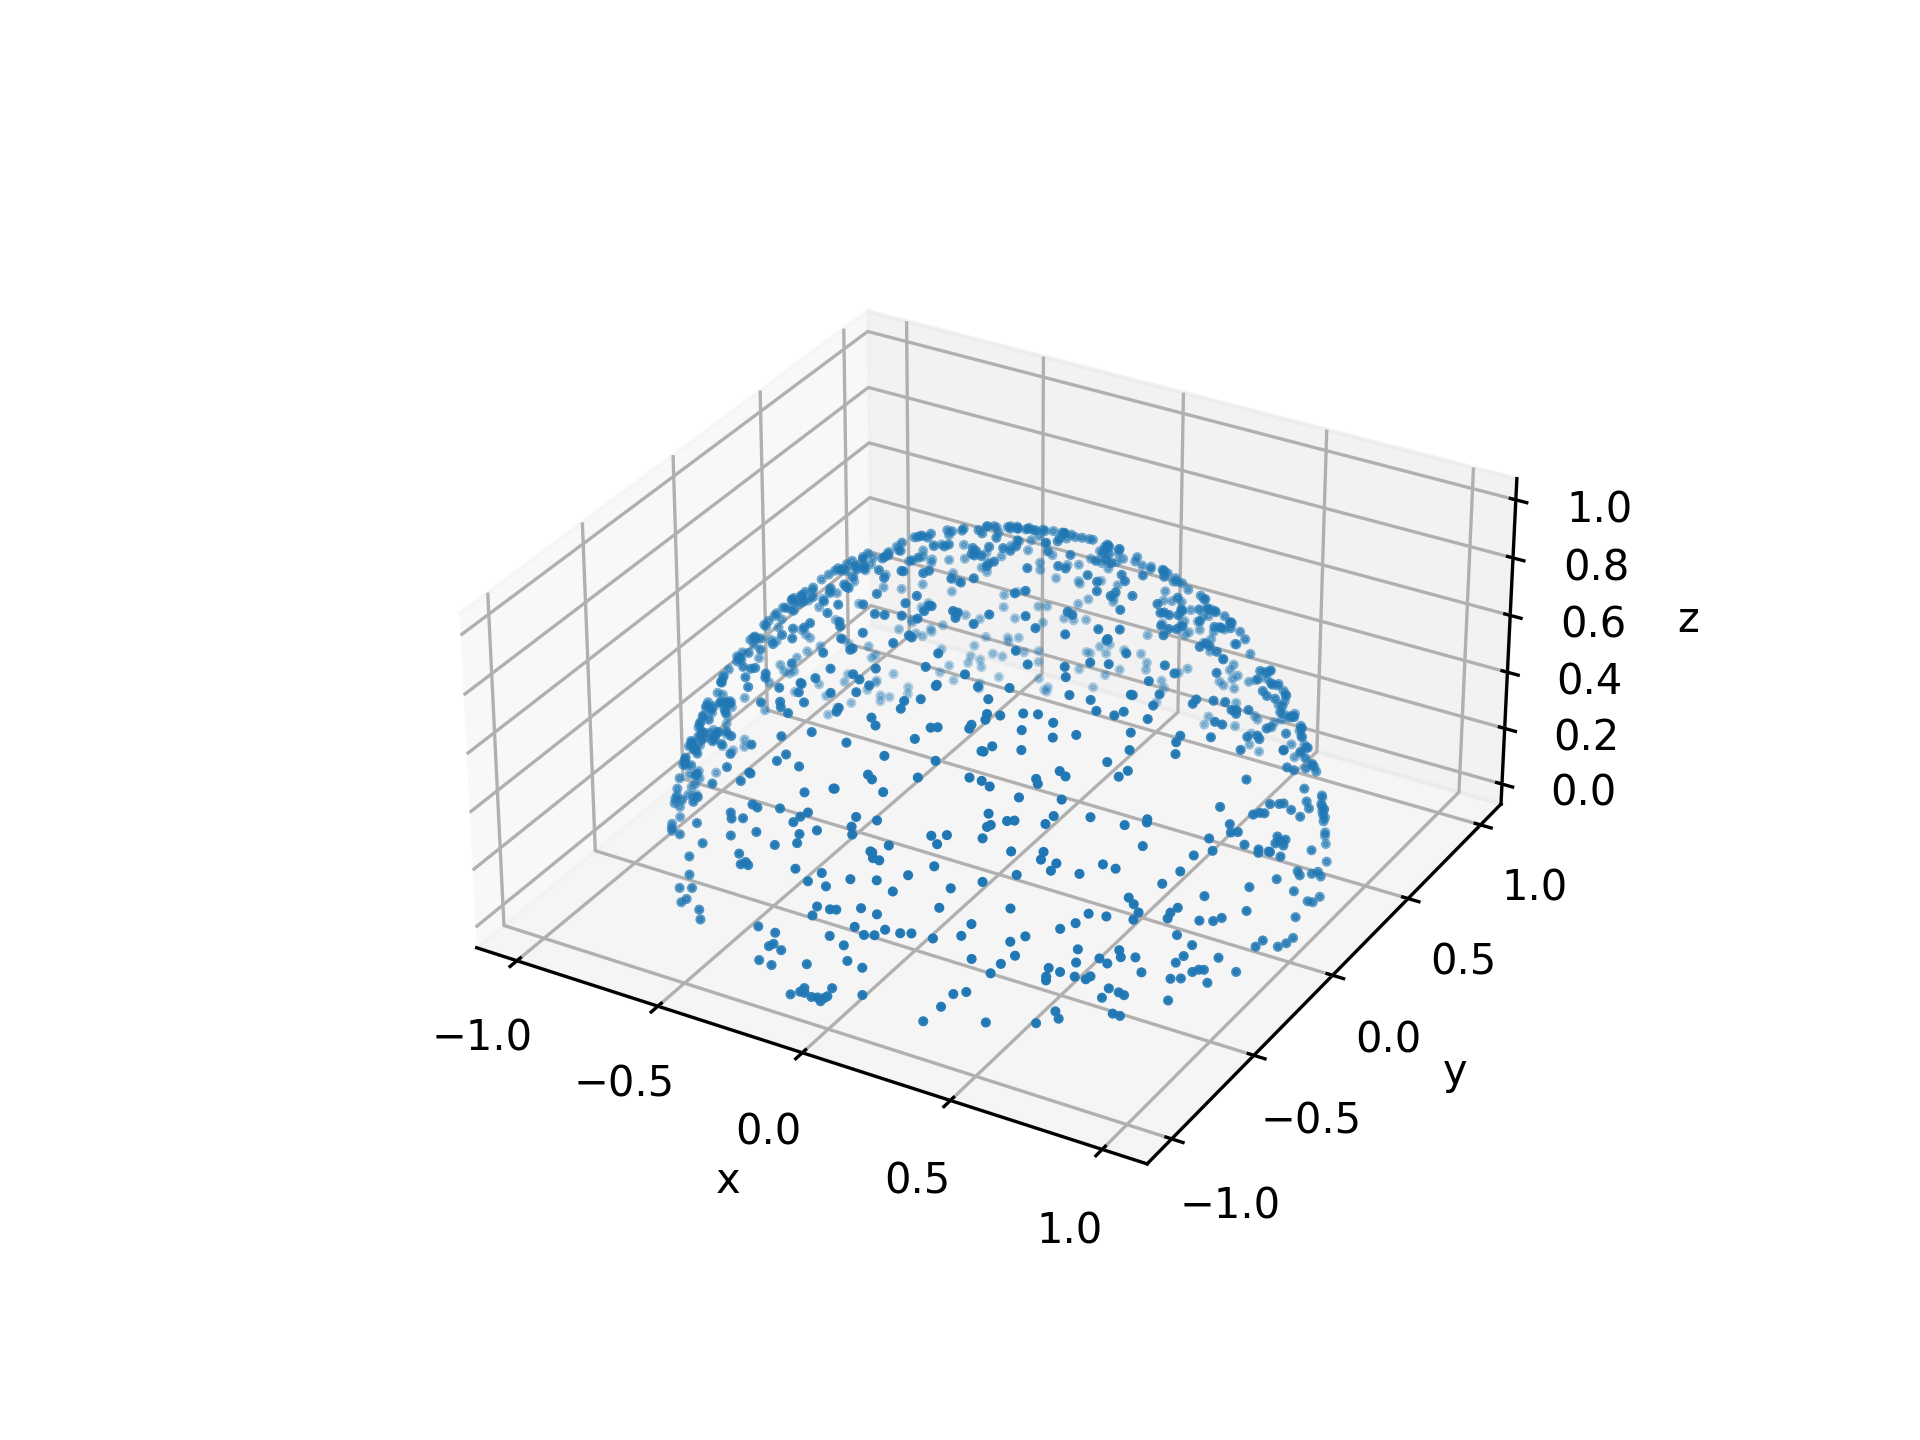
\includegraphics[width=0.5\textwidth]{fig3.png}}
    \hfill
    \subfloat[$10^4$个随机数点]{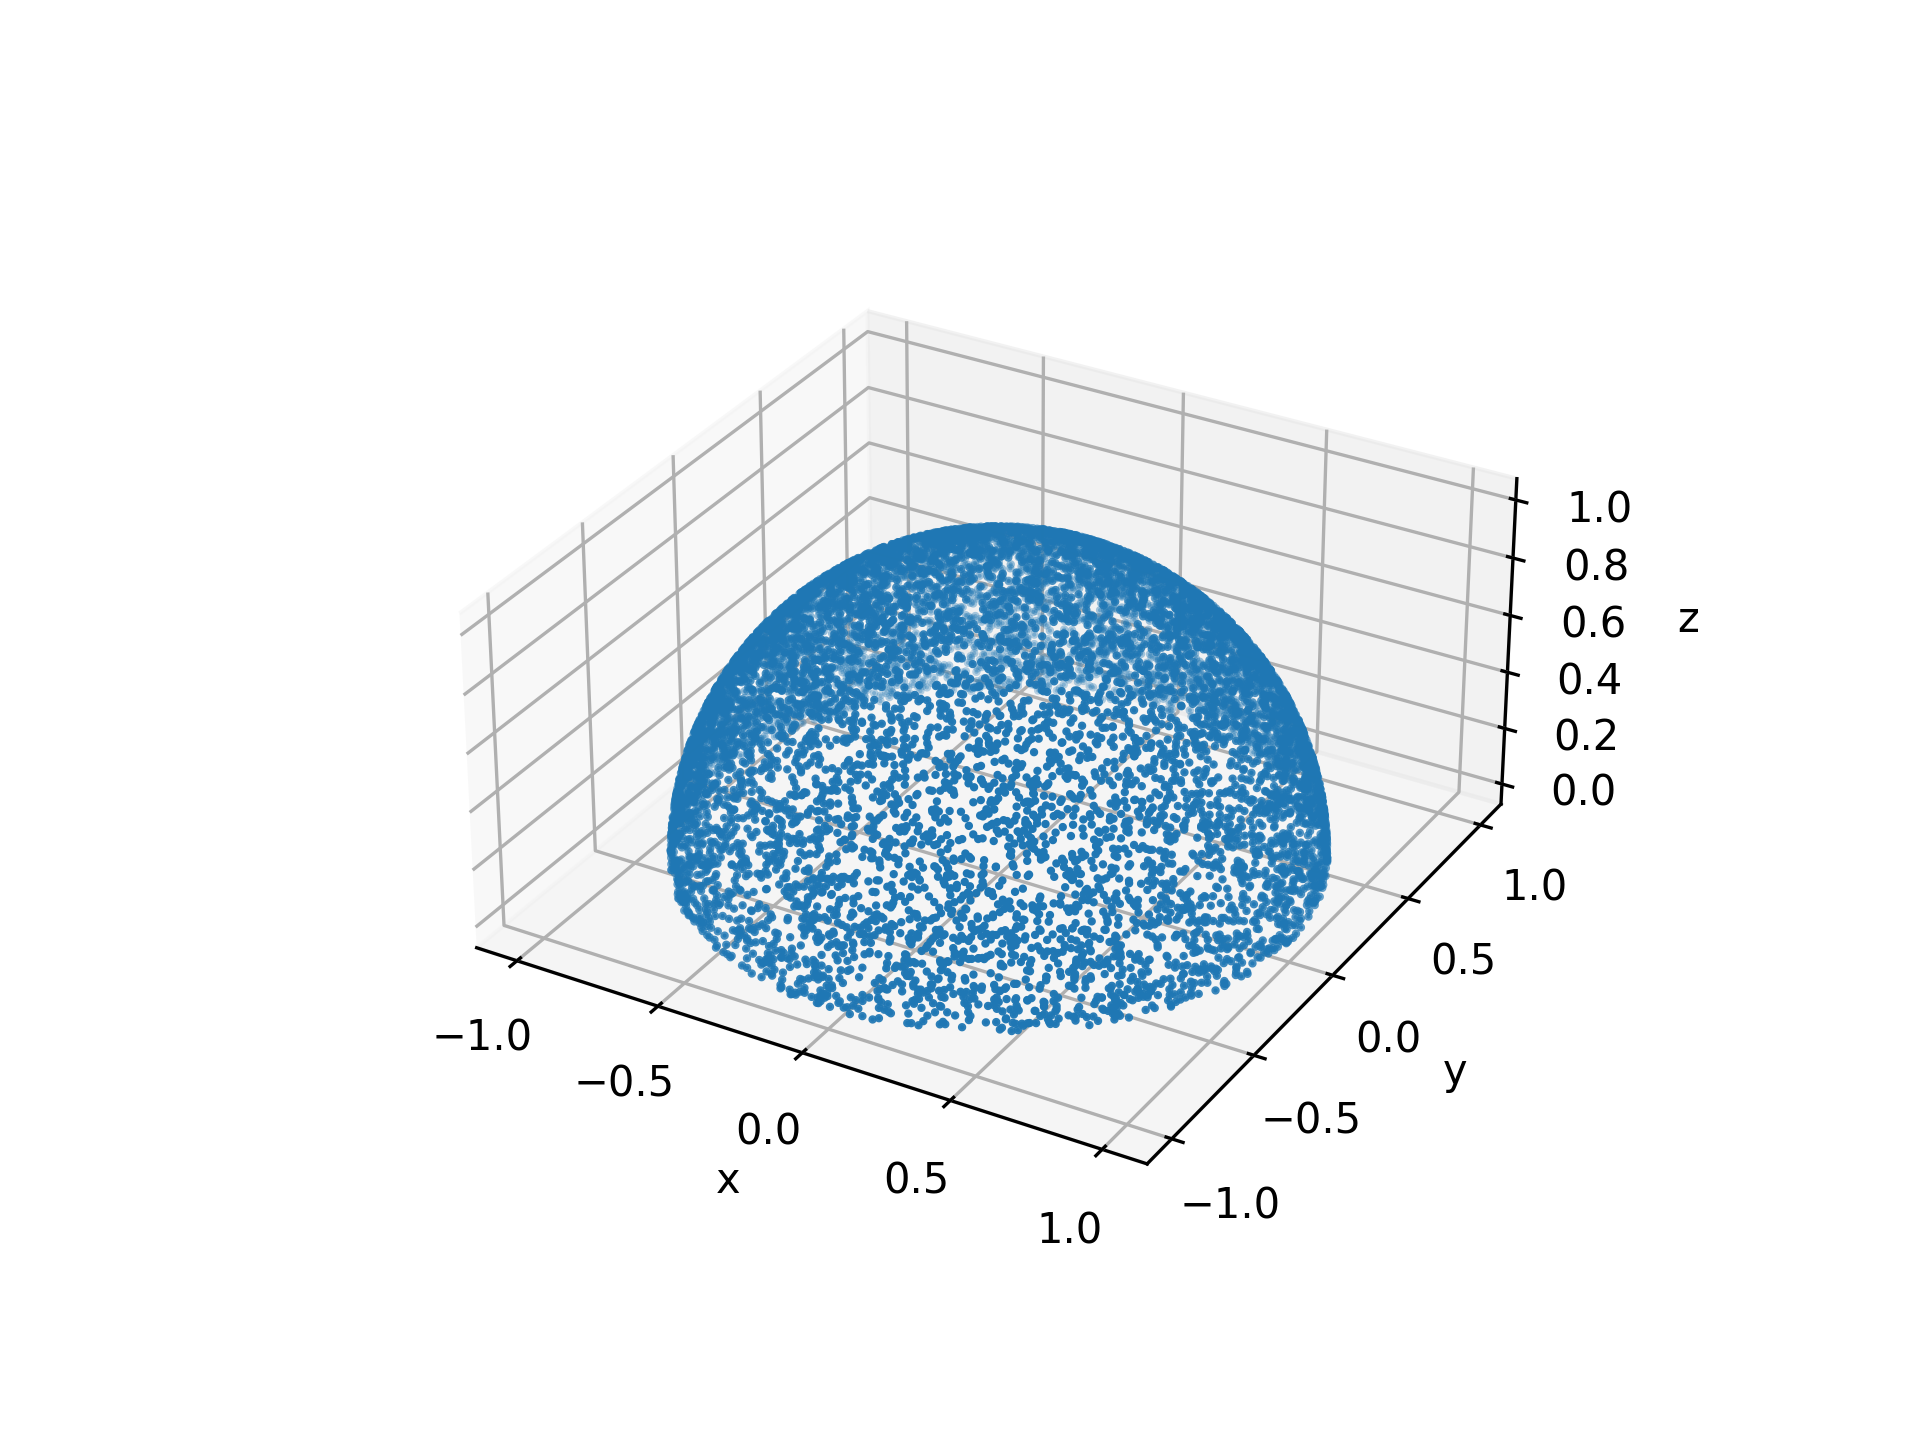
\includegraphics[width=0.5\textwidth]{fig4.png}}
    \hfill
    \subfloat[$10^5$个随机数点]{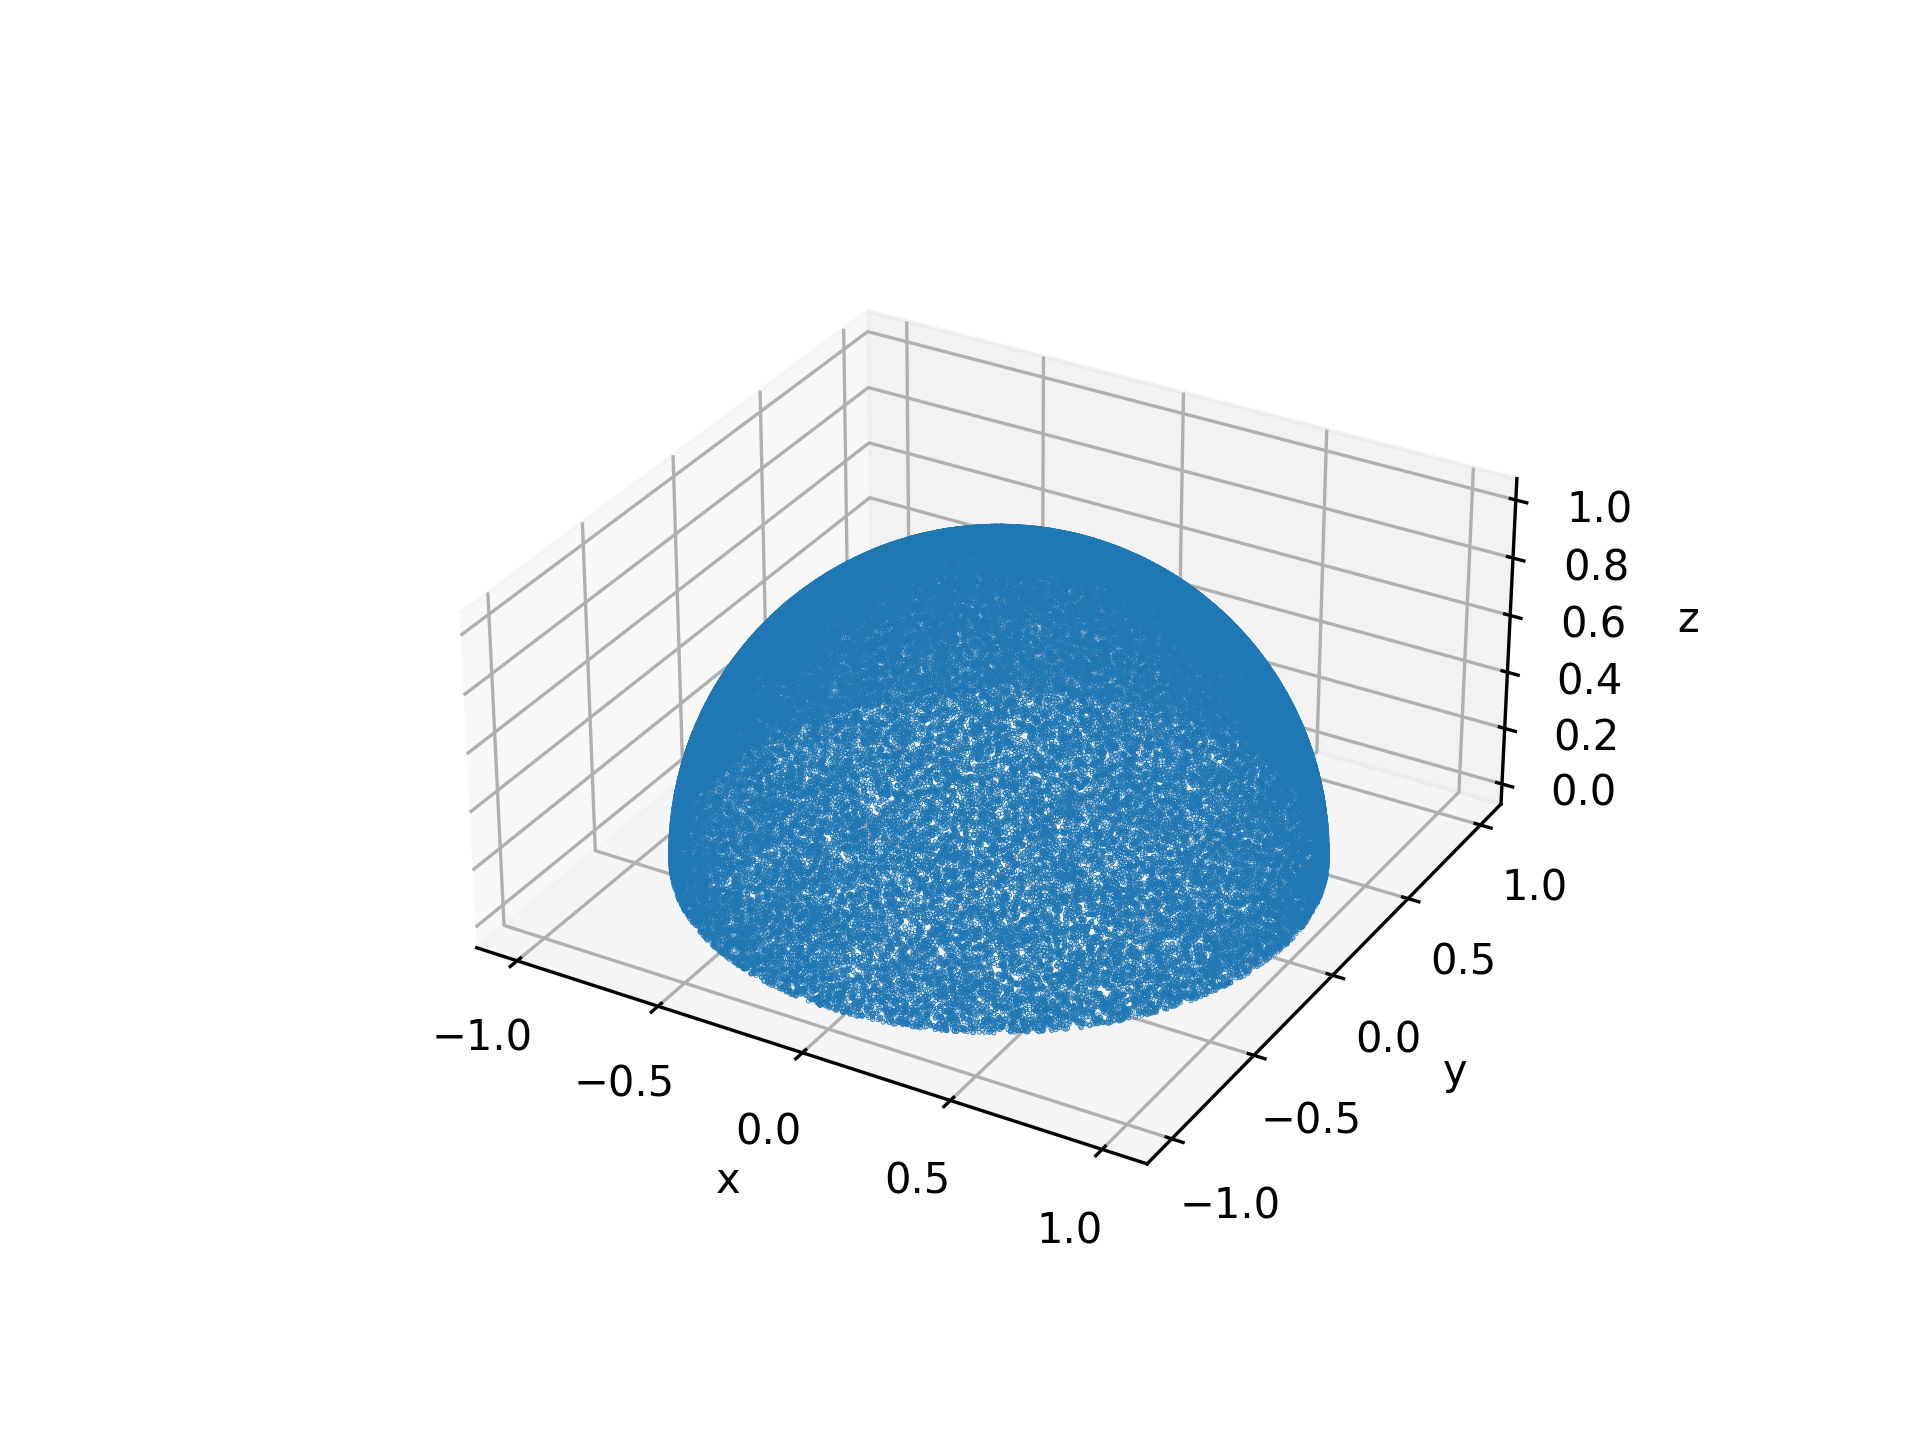
\includegraphics[width=0.5\textwidth]{fig5.png}}
    \caption{上半球面上均匀分布点散点图}
    \end{figure}

容易看出,随机数点在球面上有较好的均匀性.
\section{结论}

本题利用直接抽样法,对两组 $[0,1]$的随机数序列进行抽样分别得到球面上均匀分布的
$\theta,
\varphi$序列,并绘图进行展示,可以看出直接抽样法的优点:只要均匀分布的序列$\xi,
\eta$性质优秀,就可以保证抽样得到的结果$\theta(\xi),
\varphi(\eta)$性质一样好.但是当不能解析求反函数时这种方法不能使用,还应寻求其他的抽样方法.
\color{red} 应有定性误差分析.
\end{document}
